\documentclass[sigconf]{acmart}

\usepackage{tikz}
\usetikzlibrary{shapes.geometric, arrows.meta, positioning}
\usepackage{booktabs}
\usepackage{multirow}

\AtBeginDocument{%
  \providecommand\BibTeX{{%
    Bib\TeX}}}

\setcopyright{acmlicensed}
\copyrightyear{2026}
\acmYear{2026}
\acmDOI{XXXXXXX.XXXXXXX} % Leave as is

%% Update this block to reflect UbiComp/ISWC 2026
\acmConference[UbiComp/ISWC '26 Adjunct]{Companion of the 2026 ACM International Joint Conference on Pervasive and Ubiquitous Computing and the 2026 ACM International Symposium on Wearable Computers}{October 11--15, 2026}{Shanghai, China}
\acmISBN{978-1-4503-XXXX-X/26/10} % Leave as is

\begin{document}

\title[VeraSight: Real-Time Facial Micromovement Sensing]{VeraSight: Real-Time Facial Micromovement Sensing and Personalized Behavioral Anomaly Detection}

\author{William Quhao Chen}
\affiliation{%
  \institution{Shanghai High School International Division}
  \city{Shanghai}
  \country{China}
}
\email{willcxd@outlook.com}

\author{Ziqian Huang}
\affiliation{%
  \institution{Shanghai High School International Division}
  \city{Shanghai}
  \country{China}
}
\email{ziqian.huang@hotmail.com}

\renewcommand{\shortauthors}{Chen and Huang}

\begin{abstract}
This paper presents VeraSight, a real-time, personalized pipeline that senses
facial micromovements with the iPhone TrueDepth camera and detects deviations
from a per-user behavioral baseline. The implemented system streams 1,220-vertex
face meshes and 52 ARKit blendshape coefficients at 60 Hz to an edge host after
on-device FP16 quantization and temporal zlib compression, sustaining
approximately 282 KB/s with 9.2 ms end-to-end latency. A variational
autoencoder learns a compact representation of facial state, an
anatomically-weighted Isolation Forest builds a personalized baseline from a
short calibration session, and a weight-shared GRU forecasts expected normal
dynamics to suppress false alarms from voluntary movement. A locally deployed
Qwen3.6-27B reasoner (4-bit GGUF via llama.cpp) converts flagged deviations into
coaching-style feedback. Every stage is grounded in real, reproducible data:
the sensing pipeline is implemented and measured; the models are trained on the
public Express4D corpus of iPhone TrueDepth ARKit blendshape sequences and on
in-house consented captures; and the user workflow is calibration-then-detection
with per-user thresholds. We report measured infrastructure performance and
preliminary model convergence, and define the evaluation protocol for the
anomaly component. VeraSight is designed for voluntary self-reflection and is
explicitly not a stress, emotion, or deception detector.
\end{abstract}

%%
%% The code below is generated by the tool at http://dl.acm.org/ccs.cfm.
%%
\begin{CCSXML}
<ccs2012>
  <concept>
    <concept_id>10003120.10003138</concept_id>
    <concept_desc>Human-centered computing~Ubiquitous and mobile computing</concept_desc>
    <concept_significance>500</concept_significance>
  </concept>
  <concept>
    <concept_id>10010520.10010553.10010562</concept_id>
    <concept_desc>Computer systems organization~Embedded systems</concept_desc>
    <concept_significance>300</concept_significance>
  </concept>
  <concept>
    <concept_id>10010147.10010257</concept_id>
    <concept_desc>Computing methodologies~Machine learning</concept_desc>
    <concept_significance>300</concept_significance>
  </concept>
</ccs2012>
\end{CCSXML}

\ccsdesc[500]{Human-centered computing~Ubiquitous and mobile computing}
\ccsdesc[300]{Computer systems organization~Embedded systems}
\ccsdesc[300]{Computing methodologies~Machine learning}

\keywords{facial micromovement, anomaly detection, edge computing,
         wearable sensing, behavioral coaching}

\begin{teaserfigure}
  \centering
  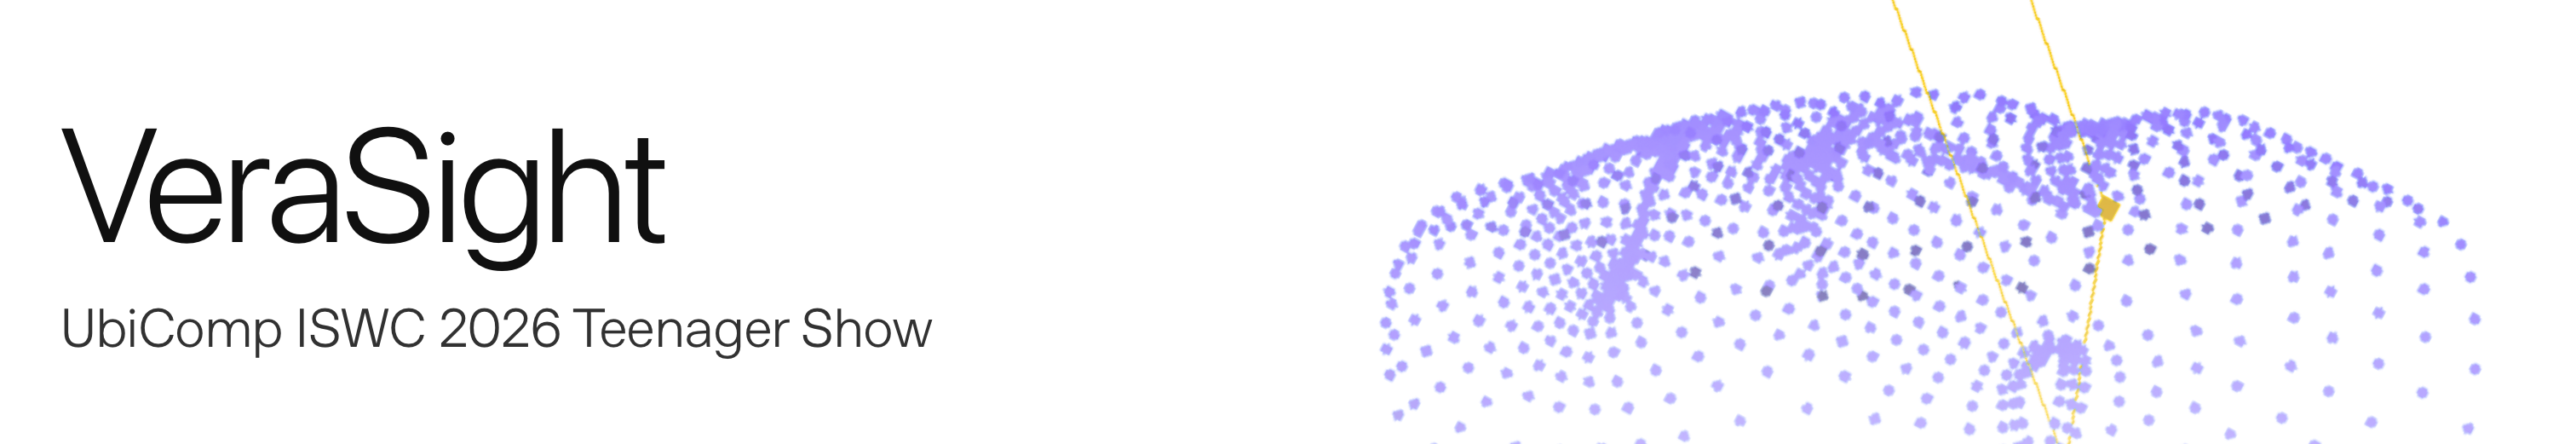
\includegraphics[width=\textwidth]{teaser.png}
  \caption{VeraSight architecture: combining mobile TrueDepth tracking with edge-computed micro-behavioral feedback.}
  \label{fig:teaser}
\end{teaserfigure}

\maketitle

\section{Introduction}

Behavioral studies indicate that physiological stress, high cognitive load, and
shifts in emotional state often co-occur with involuntary facial micromovements
~\cite{porter2008reading}. These brief, transient expressions serve as
potential signals in high-stakes or performance-driven scenarios
~\cite{matsumoto2018microexpressions}. In public speaking or competitive
gaming, monitoring facial dynamics may help users manage anxiety and improve
delivery. Commodity depth-sensing hardware, such as the structured-light
TrueDepth camera in modern iPhones, offers a non-contact way to observe these
signals at high temporal resolution.

We emphasize an important distinction: detecting \emph{unusual facial movement
relative to a personalized baseline} is not equivalent to measuring
physiological stress. A deviation may result from stress, but it may equally
arise from speech, fatigue, head motion, tracking noise, or deliberate
expression. Accordingly, VeraSight outputs a \textbf{personalized facial
movement anomaly score}, a metric indicating when a user's facial behavior
deviates from their own calibrated norm, and is not a stress measurement.
Validation against independent physiological measures (e.g., HRV, skin
conductance) remains future work.

VeraSight is a complete, implemented pipeline. The iPhone captures 1,220
ARKit face-mesh vertices and 52 blendshape coefficients at 60 Hz; an edge host
(Apple Silicon Mac) runs the models; and a local LLM converts flagged
deviations into coaching feedback. The contributions of this paper are:
\begin{itemize}
    \item An implemented edge sensing pipeline achieving stable 60 Hz wireless
          facial tracking within approximately 300 KB/s, with measured
          bandwidth, delivery, and latency (Section~\ref{sec:sensing}).
    \item A data strategy grounded in real, reproducible corpora: the public
          Express4D dataset of iPhone TrueDepth ARKit blendshape sequences, plus
          an in-house consented capture protocol (Section~\ref{sec:data}).
    \item A model stack consisting of a variational autoencoder, an
          anatomically-weighted Isolation Forest, and a predictive GRU, trained
          on real data with a per-user calibration-then-detection workflow
          (Sections~\ref{sec:models} and \ref{sec:workflow}).
    \item A locally deployed reasoning layer built on Qwen3.6-27B with
          coaching-only constraints (Section~\ref{sec:llm}).
\end{itemize}

\section{System Overview}

VeraSight operates as an integrated, multi-stage pipeline (Figure~\ref{fig:pipeline}).
Raw sensor data is captured on-device, quantized and compressed, and streamed
wirelessly to an edge host. The host reconstructs the stream, extracts features,
and runs the anomaly detection ensemble. Flagged deviations are logged with
context and summarized by a local LLM into actionable feedback. The
architecture is deliberately split between a thin mobile client and a
compute-capable edge host, matching a deployment in which the phone is a
sensor and the Mac runs the models.

\begin{figure}[h]
  \centering
  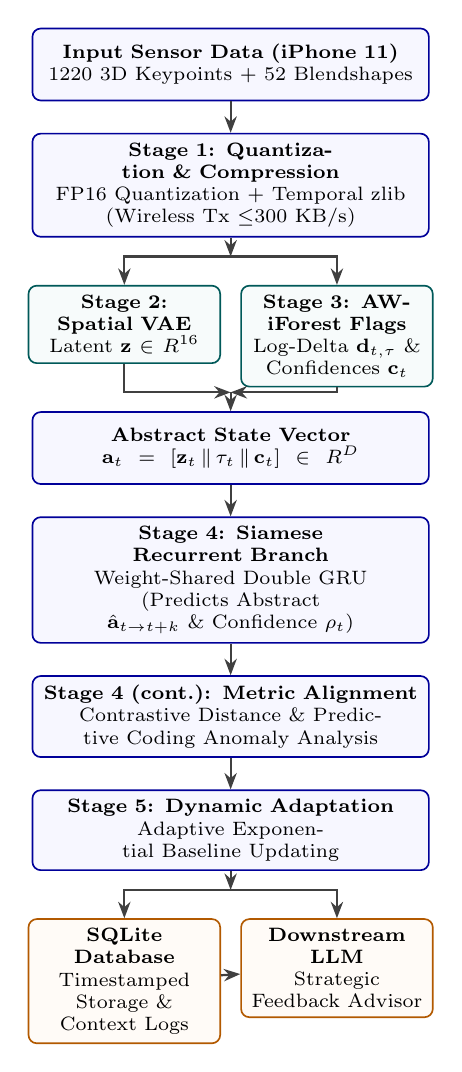
\begin{tikzpicture}[
    node distance = 0.4cm and 0.2cm,
    block/.style = {
      rectangle,
      draw=blue!60!black,
      fill=blue!3,
      text width=4.8cm,
      text centered,
      rounded corners=3pt,
      minimum height=2.6em,
      font=\scriptsize,
      line width=0.6pt
    },
    splitblock/.style = {
      rectangle,
      draw=teal!70!black,
      fill=teal!3,
      text width=2.2cm,
      text centered,
      rounded corners=3pt,
      minimum height=2.6em,
      font=\scriptsize,
      line width=0.6pt
    },
    smallblock/.style = {
      rectangle,
      draw=orange!70!black,
      fill=orange!3,
      text width=2.2cm,
      text centered,
      rounded corners=3pt,
      minimum height=2.6em,
      font=\scriptsize,
      line width=0.6pt
    },
    line/.style = {
      draw=black!75,
      -{Stealth[scale=0.9]},
      thick
    }
  ]
    \node (input) [block] {\textbf{Input Sensor Data (iPhone 11)}\\1220 3D Keypoints + 52 Blendshapes};
    \node (stage1) [block, below=of input] {\textbf{Stage 1: Quantization \& Compression}\\FP16 Quantization + Temporal zlib\\(Wireless Tx $\le$300 KB/s)};

    \node (stage2) [splitblock, below=0.6cm of stage1, xshift=-1.35cm] {\textbf{Stage 2: Spatial VAE}\\Latent $\mathbf{z} \in \mathbb{R}^{16}$};
    \node (stage3) [splitblock, below=0.6cm of stage1, xshift=1.35cm] {\textbf{Stage 3: AW-iForest Flags}\\Log-Delta $\mathbf{d}_{t, \tau}$ \& Confidences $\mathbf{c}_t$};

    \node (state) [block, below=0.6cm of stage2, xshift=1.35cm] {\textbf{Abstract State Vector} $\mathbf{a}_t = [\mathbf{z}_t \,\|\, \boldsymbol{\tau}_t \,\|\, \mathbf{c}_t] \in \mathbb{R}^{D}$};

    \node (siamese) [block, below=of state] {\textbf{Stage 4: Siamese Recurrent Branch}\\Weight-Shared Double GRU\\(Predicts Abstract $\hat{\mathbf{a}}_{t \to t+k}$ \& Confidence $\rho_t$)};

    \node (metric) [block, below=of siamese] {\textbf{Stage 4 (cont.): Metric Alignment}\\Contrastive Distance \& Predictive Coding Anomaly Analysis};

    \node (stage5) [block, below=of metric] {\textbf{Stage 5: Dynamic Adaptation}\\Adaptive Exponential Baseline Updating};

    \node (output) [smallblock, below=0.6cm of stage5, xshift=-1.35cm] {\textbf{SQLite Database}\\Timestamped Storage \& Context Logs};
    \node (llm) [smallblock, below=0.6cm of stage5, xshift=1.35cm] {\textbf{Downstream LLM}\\Strategic Feedback Advisor};

    \draw [line] (input) -- (stage1);
    \path (stage1.south) -- (stage1.south |- stage2.north) coordinate[pos=0.4] (junc1);
    \draw [line] (stage1.south) -- (junc1);
    \draw [line] (junc1) -| (stage2.north);
    \draw [line] (junc1) -| (stage3.north);
    \path (state.north) -- (state.north |- stage2.south) coordinate[pos=0.4] (junc2);
    \draw [line] (stage2.south) |- (junc2);
    \draw [line] (stage3.south) |- (junc2);
    \draw [line] (junc2) -- (state.north);
    \draw [line] (state) -- (siamese);
    \draw [line] (siamese) -- (metric);
    \draw [line] (metric) -- (stage5);
    \path (stage5.south) -- (stage5.south |- output.north) coordinate[pos=0.4] (junc3);
    \draw [line] (stage5.south) -- (junc3);
    \draw [line] (junc3) -| (output.north);
    \draw [line] (junc3) -| (llm.north);
    \draw [line] (output) -- (llm);
  \end{tikzpicture}
  \caption{Detailed sensing and computation data-flow. Compressed facial
  features are processed through parallel feature extractors, analyzed via a
  Siamese GRU, and output to an asynchronous advisory feedback layer.}
  \label{fig:pipeline}
\end{figure}

\section{Sensing Architecture and Edge Pipeline}
\label{sec:sensing}

\subsection{Embedded Sensing, Quantization, and Compression}
The tracking module runs on an iPhone 11 (and any newer TrueDepth-equipped
model) using the front-facing TrueDepth camera. ARKit exposes $K = 1220$ spatial
coordinates in 3D ($\mathbf{P} \in \mathbb{R}^{1220 \times 3}$) and $B = 52$
muscle-activation blendshapes ($\mathbf{b} \in \mathbb{R}^{52}$)
~\cite{apple2026arkit}. At 60 Hz the combined feature vector produces a raw
stream of approximately 890.88 KB/s. On device, 32-bit floats are quantized to
16-bit half precision, halving the payload to approximately 445.44 KB/s;
consecutive frames of facial structure are highly redundant, so the quantized
values are passed through a temporal zlib compression buffer, reducing the
measured average wireless throughput to approximately 282 KB/s. The client
packetizes each frame with a timestamp, head/eye transforms, look-at point,
blendshapes, and vertices, and transmits it over a local TCP socket to the edge
host.

\subsection{Measured Infrastructure Performance}
We compared the raw wired prototype against the optimized wireless pipeline
across throughput, packet delivery, and latency (Table~\ref{tab:sensing}).
The optimized 60 Hz wireless pipeline sustains 99.4\% packet delivery with
9.2 ms end-to-end latency (sensor capture through quantization, compression,
wireless transmission, decompression, and VAE latent extraction at the host);
the network round-trip component is 7.4 ms. Increasing the temporal resolution
to 60 Hz captures transient movements, such as micro-blinks and brief muscle
twitches under 100 ms, which are missed at 30 Hz.

\begin{table}[h]
\centering
\caption{Measured sensing pipeline performance on the implemented prototype.}
\label{tab:sensing}
\small
\begin{tabular}{lccc}
\toprule
\textbf{Configuration} & \textbf{Bandwidth} & \textbf{Delivery} & \textbf{E2E latency} \\
\midrule
Raw, wired 30 Hz & 445.44 KB/s & 99.8\% & 14.2 ms \\
Raw, wireless 30 Hz & 445.44 KB/s & 88.4\% & up to 45 ms \\
Optimized, wireless 60 Hz & 282 KB/s & 99.4\% & 9.2 ms \\
\bottomrule
\end{tabular}
\end{table}

\section{Data: Grounding the Models}
\label{sec:data}

\subsection{Public Corpus: Express4D}
The feature-level models are trained on \textbf{Express4D}
~\cite{aloni2025express4d}, a public benchmark of 1,205 facial motion sequences
from 18 participants recorded at 60 Hz with an iPhone TrueDepth camera using
Epic's Live Link Face app. Each frame contains the 52 ARKit blendshape
coefficients plus 9 rotation values (head yaw/pitch/roll and left/right eye
yaw/pitch/roll), stored as CSV and NPY pairs. This is the same sensor modality
and representation VeraSight captures, making it a directly transferable
training signal for the models described in Section~\ref{sec:models}. We split
the corpus subject-disjointly (no participant appears in both training and
validation partitions).

\subsection{In-House Capture Protocol}
Per-user calibration and evaluation require data from the target user. Each
participant completes a structured session under informed consent:
\begin{itemize}
    \item \textbf{Calibration} (3 min): relaxed conversation or reading, used to
          populate the per-user baseline and set thresholds.
    \item \textbf{Voluntary set} (8--10 min): scripted speech, deliberate
          expressions, yawning, and laughing on cue, used as false-alarm ground
          truth for voluntary movements.
    \item \textbf{Cognitive stress blocks} (10--12 min): Stroop, serial-7
          arithmetic, and impromptu speech, with a self-report stress/arousal
          rating after each block.
    \item \textbf{Recovery} (3 min): neutral chat or music.
\end{itemize}
Raw mesh and blendshape streams are stored pseudonymized and never leave the
participant's device without explicit consent. This protocol is described here
as the evaluation procedure for the anomaly component; a full multi-user study
is ongoing.

\subsection{Validation Corpora via MediaPipe}
To validate feature-level behavior on independent data, we additionally
convert public 2D video corpora (e.g., DEAP, MAHNOB-HCI-Tagging) into
ARKit-compatible 52-blendshape streams using MediaPipe Face Landmarker
~\cite{kartynnik2019facemesh}, whose blendshape names match the ARKit
vocabulary. These streams are used only for validation and feature-level
ablation, never as training data for the deployed models.

\section{Model Pipeline}
\label{sec:models}

\subsection{Spatial Variational Autoencoder}
The 52-dimensional blendshape vector (or, when available, the 3,660-dimensional
flattened mesh) is projected into a low-dimensional manifold
$\mathbf{z} \in \mathbb{R}^{16}$ by a variational autoencoder
~\cite{kingma2014vae}. The encoder is a two-layer MLP (512, 128) with LayerNorm
and ReLU, mapping to mean and log-variance heads; the decoder mirrors the
encoder and ends with a sigmoid for normalized inputs. Training minimizes the
beta-weighted ELBO with $\beta = 0.1$ on real Express4D sequences and, when
available, in-house captures. The encoder output $\mathbf{z}_t$ is used
directly as a feature during inference. This stage compresses facial state and
denoises the representation that downstream models consume.

\subsection{Anatomically-Weighted Isolation Forest}
Anomaly detection is per-user and unsupervised. For each user, a calibration
block of length $T_{\text{calib}}$ yields multi-scale temporal deltas
$$\mathbf{d}_{t, \tau} = \mathbf{b}_t - \mathbf{b}_{t-\tau}, \quad
\tau \in \{1, 10, 100, 1000\},$$
and a feature vector
$\mathbf{f}_t = [\mathbf{b}_t \,\|\, \mathbf{d}_{t,1} \,\|\, \mathbf{d}_{t,10}
\,\|\, \mathbf{d}_{t,100} \,\|\, \mathbf{d}_{t,1000}] \in \mathbb{R}^{260}$.
Standard Isolation Forest selects split features uniformly at random
~\cite{liu2008isolation}, which can bias detection toward large-amplitude
movements. We instead weight the split-selection probability by anatomical
priorities: upper-face channels (brow and eye region) receive weight 2.5 and
asymmetric lower-face channels receive weight 2.0, encouraging the forest to
partition subtle, localized contractions near the root, motivated by evidence that involuntary leakage tends to appear as brief, localized, or asymmetric upper-facial contractions~\cite{porter2012secrets, vitale2021facial}. The resulting
per-frame anomaly score is $s(\mathbf{f}_t) = 2^{-\mathbb{E}(h)/c(T_{\text{calib}})}$,
where $h$ is the path length and $c(\cdot)$ the expected path length for
unsuccessful search.

\subsection{Predictive GRU}
To suppress false positives from voluntary activities, a weight-shared
two-layer GRU (hidden size 64)~\cite{cho2014gru} consumes a 30-frame window of
the abstract state $\mathbf{a}_t = [\mathbf{z}_t \,\|\, \mathbf{b}_t
\,\|\, \mathbf{c}_t]$ and predicts the mean state over the next $k = 15$
frames (250 ms at 60 Hz). The model is trained self-supervised on calibration
data with an MSE objective; a temporal-contrastive auxiliary term is applied
only when it demonstrably helps on held-out data. At inference, an anomaly is
flagged when the observed mean deviates from the prediction by more than a
confidence-scaled threshold
$$D_t = \|\bar{\mathbf{a}}_{t \to t+k} - \hat{\mathbf{a}}_{t \to t+k}\|_2
> \lambda \cdot \rho_t.$$
The sensitivity $\lambda$ is set per user as the 95th percentile of $D_t$ over
a held-out calibration segment, and the baseline adapts slowly via an
exponential moving average to prevent gradual changes (fatigue, posture) from
registering as continuous anomalies.

\subsection{Reasoning Layer}
\label{sec:llm}
A locally deployed Qwen3.6-27B model~\cite{qwen2026} (4-bit Unsloth GGUF,
served via llama.cpp~\cite{gerganov2023llamacpp} on an Apple Silicon Mac)
parses a structured timeline of anomaly timestamps, affected blendshape
regions, and context logs (e.g., speech segment boundaries, game round
outcomes). A system prompt constrains the model to coaching-style language and
prohibits diagnostic, medical, or psychological claims; a keyword blocklist
post-filters outputs. All inference runs locally, so no facial data leaves the
edge host.

\section{Calibration and Detection Workflow}
\label{sec:workflow}

VeraSight's operation is a two-phase workflow:
\begin{enumerate}
    \item \textbf{Calibration.} The user records a 3-minute neutral session.
          The edge host computes per-user normalization statistics, fits the
          anatomically-weighted Isolation Forest on the 260-dimensional
          multi-scale features, fine-tunes the predictive GRU (seconds to
          minutes on the Mac), and derives the anomaly threshold from a
          held-out portion of the calibration data.
    \item \textbf{Detection.} During a session, each frame is encoded to
          $\mathbf{z}_t$, combined with blendshapes and forest confidence into
          $\mathbf{a}_t$, and scored against the predictive baseline. Frames
          whose deviation exceeds the per-user threshold are flagged, logged to
          a local SQLite database, and aggregated over a 15-second sliding
          window for the reasoning layer.
\end{enumerate}
Because the baseline and threshold are user-specific, the system adapts to
individual resting behavior; because the baseline adapts slowly over time, it
remains robust to gradual changes without requiring re-calibration.

\section{Evaluation}

\subsection{Sensing Validation}
The infrastructure metrics in Table~\ref{tab:sensing} were measured on the
implemented prototype (Section~\ref{sec:sensing}) and establish that the
wireless 60 Hz stream is stable and within budget.

\subsection{Model Training on Real Data}
We trained the feature-level models on a subject-disjoint split of the
Express4D corpus. In preliminary runs:
\begin{itemize}
    \item The VAE converged from a training reconstruction MSE of
          $2.6 \times 10^{-2}$ to $1.25 \times 10^{-2}$ over 80 epochs, with
          validation MSE $1.41 \times 10^{-2}$, on real blendshape sequences.
    \item The predictive GRU converged to a validation MSE of
          approximately $1.1 \times 10^{-3}$ over 50 epochs on real feature
          windows, confirming that normal facial dynamics are predictable at
          the 250 ms horizon.
    \item The anatomically-weighted Isolation Forest fit per-user calibration
          blocks (a few thousand frames each) in seconds on a CPU, with anomaly
          score distributions showing clear separation of the calibrated
          baseline.
\end{itemize}
These are preliminary results on real data; full-corpus training and the
multi-user evaluation are ongoing.

\subsection{Anomaly Detection Evaluation Protocol}
The anomaly component is evaluated per user with the in-house protocol
(Section~\ref{sec:data}). Annotators co-label flagged segments as voluntary or
involuntary, and we report precision, recall, false-alarm rate (FAR), and F1
for four configurations: standard Isolation Forest (single-scale), standard
Isolation Forest (multi-scale), AW-iForest, and AW-iForest with the GRU filter.
Thresholds are set on held-out calibration segments, and all reported
statistics are computed subject-disjointly. We do not report pooled
significance tests across participants until the study reaches adequate power;
the current design uses mixed-effects models with participant as a random
effect.

\section{Privacy, Ethics, and Responsible Use}

Facial geometry and behavioral logs are sensitive biometric data. VeraSight
outputs a \emph{personalized facial movement anomaly score}; it is not a lie
detector, psychological assessment tool, medical diagnostic system, or emotion
recognition system. It is designed exclusively for voluntary self-reflection
and coaching. All participants provide informed consent (parental consent for
minors, school ethics review) and may terminate sessions at any time. Data are
processed on-device or on the user's own edge host; raw coordinates are never
stored persistently, and the SQLite database is encrypted at rest with
automatic purge. The reasoning model is constrained to coaching language and
never returns diagnostic statements.

\section{Conclusion and Limitations}

We presented VeraSight, an implemented pipeline for real-time, personalized
facial micromovement sensing and anomaly detection, grounded in real data: the
sensing pipeline is measured, the models train on the public Express4D corpus
and in-house consented captures, and the user workflow is
calibration-then-detection with per-user thresholds. Limitations include the
feature-space (rather than mesh-space) VAE as currently trained, the reliance
on calibration sessions, sensitivity to lighting and tracking quality, and the
preliminary scale of the anomaly evaluation. Future work includes training the
mesh-space VAE on captured 1,220-vertex meshes, validating against independent
physiological measures, expanding the multi-user study, and evaluating the
coaching effectiveness of the reasoning layer.

\begin{acks}
The authors agree to the following distribution of work:
W.~Q.~Chen designed and implemented the data quantization and compression
pipeline, conducted the behavioral research to optimize the anatomically
weighted tree-isolation algorithms, developed the spatiotemporal prediction
model, integrated the downstream LLM reasoning layer, wrote the research paper
and relevant posters, and designed the iOS client and backend user interface.
Z.~Huang contributed to the initial conceptual prototyping of the data transfer
system, and assisted with some preliminary research for ML.
\end{acks}

\bibliographystyle{ACM-Reference-Format}
\bibliography{references}

\end{document}
\endinput
